\documentclass[12pt]{article}
\usepackage[a4paper, total={6in, 9in}]{geometry}
\usepackage{graphicx}
\graphicspath{ {./images/output/} }
\usepackage{caption}
\usepackage[english]{babel}
\usepackage{titling}
\usepackage{float}
% \usepackage{amsmath}
% \usepackage{minted}
% \usepackage{multicol}
% \usepackage{array}
% \usepackage{setspace}
% \usepackage{placeins}
% \usepackage{hyperref}
\setlength{\parindent}{0pt}

% \usepackage{lipsum}

\title{Drawing Line Diagrams in AutoCAD Electrical.}
\author{}
\date{}

\pagenumbering{gobble}
\begin{document}
\vspace*{\fill}
\begin{center}

    \emph{Heaven's Light is Our Guide} \\
    \textbf{Rajshahi University of Engineering and Technology} \\

    \begin{figure}[H]
        \centering
        
\includegraphics[scale=.34]{images/RUET_logo.png}
        \label{fig:ruet_logo}
    \end{figure}
    \vspace{5mm}

    \textbf{Course Code}\\
    ECE 3200\\
    \vspace{3mm}
    \textbf{Course Title}\\
    Electrical Services Design

    \vspace{5mm}
    \textbf{Experiment Date:} {February 4, 2025}\\
    \textbf{Submission Date:} {February 18, 2025}\\

    \vspace{5mm}
    \textbf{Lab Report 5: \\ Implementation of Parametric \& Full Units PLC: Insertion, Editing, \& Modification.}

    \vspace{15mm}

    \begin{tabular}{c|c}
        \textbf{Submitted to} & \textbf{Submitted by} \\
        Md. Faysal Ahamed     &                       \\
        Lecturer              &                       \\
        Dept of ECE, RUET     & Md. Tajim An Noor     \\
        -                     & Roll: 2010025         \\
        Moloy Kumar Ghosh     &                       \\
        Lecturer              &                       \\
        Dept of ECE, RUET     &                       \\
    \end{tabular}

\end{center}
\vspace*{\fill}


\pagebreak

\tableofcontents

\pagebreak
\pagenumbering{arabic}
\maketitle

\section*{Introduction}
\addcontentsline{toc}{section}{Introduction}
A Programmable Logic Controller (PLC) is an industrial computer used to control automated processes, managing inputs and outputs based on pre-programmed instructions \cite{johnson2006introduction}. PLCs are valued for their reliability, scalability, and real-time processing.

A Parametric PLC allows dynamic configuration of system parameters like timers, counters, and I/O addresses, making it adaptable to various needs \cite{clarke2005practical}. This flexibility is useful for applications requiring frequent adjustments.

A Full Units PLC integrates all essential modules, including CPU, I/O, power supply, and communication interfaces, for comprehensive automation solutions \cite{bolton2015programmable}.

Working with a Parametric PLC involves:
\begin{itemize}
    \item Inserting: Integrating the PLC into a project with defined configurations.
    \item Editing: Adjusting parameters to optimize performance.
    \item Modifying: Changing program structures and logic flow as needed.
\end{itemize}

Mastering these processes enables engineers to design efficient and customizable automation systems.

\section*{Required Equipment/Software}
\addcontentsline{toc}{section}{Required Equipment/Software}
\begin{itemize}
    \item AutoCAD Electrical
    \item \LaTeX{} for report writing
\end{itemize}

\section*{Procedure}
\addcontentsline{toc}{section}{Procedure}
\begin{enumerate}
    \item \textbf{Inserting Parametric \& Full Units PLC}
          \begin{enumerate}
              \item Create a new project in the PLC software.
              \item Select the PLC model and configuration.
              \item Insert the Parametric PLC module.
              \item Define I/O addresses and set parameters.
              \item Compile and upload the configuration.
          \end{enumerate}
    \item \textbf{Editing \& Modifying Parametric PLC}
          \begin{enumerate}
              \item Open the existing project file.
              \item Modify parameters like timers and counters.
              \item Adjust I/O mapping if needed.
              \item Simulate changes before deployment.
              \item Save and download the modified program.
              \item Monitor performance using debugging tools.
          \end{enumerate}
\end{enumerate}

\begin{figure}[H]
    \centering
    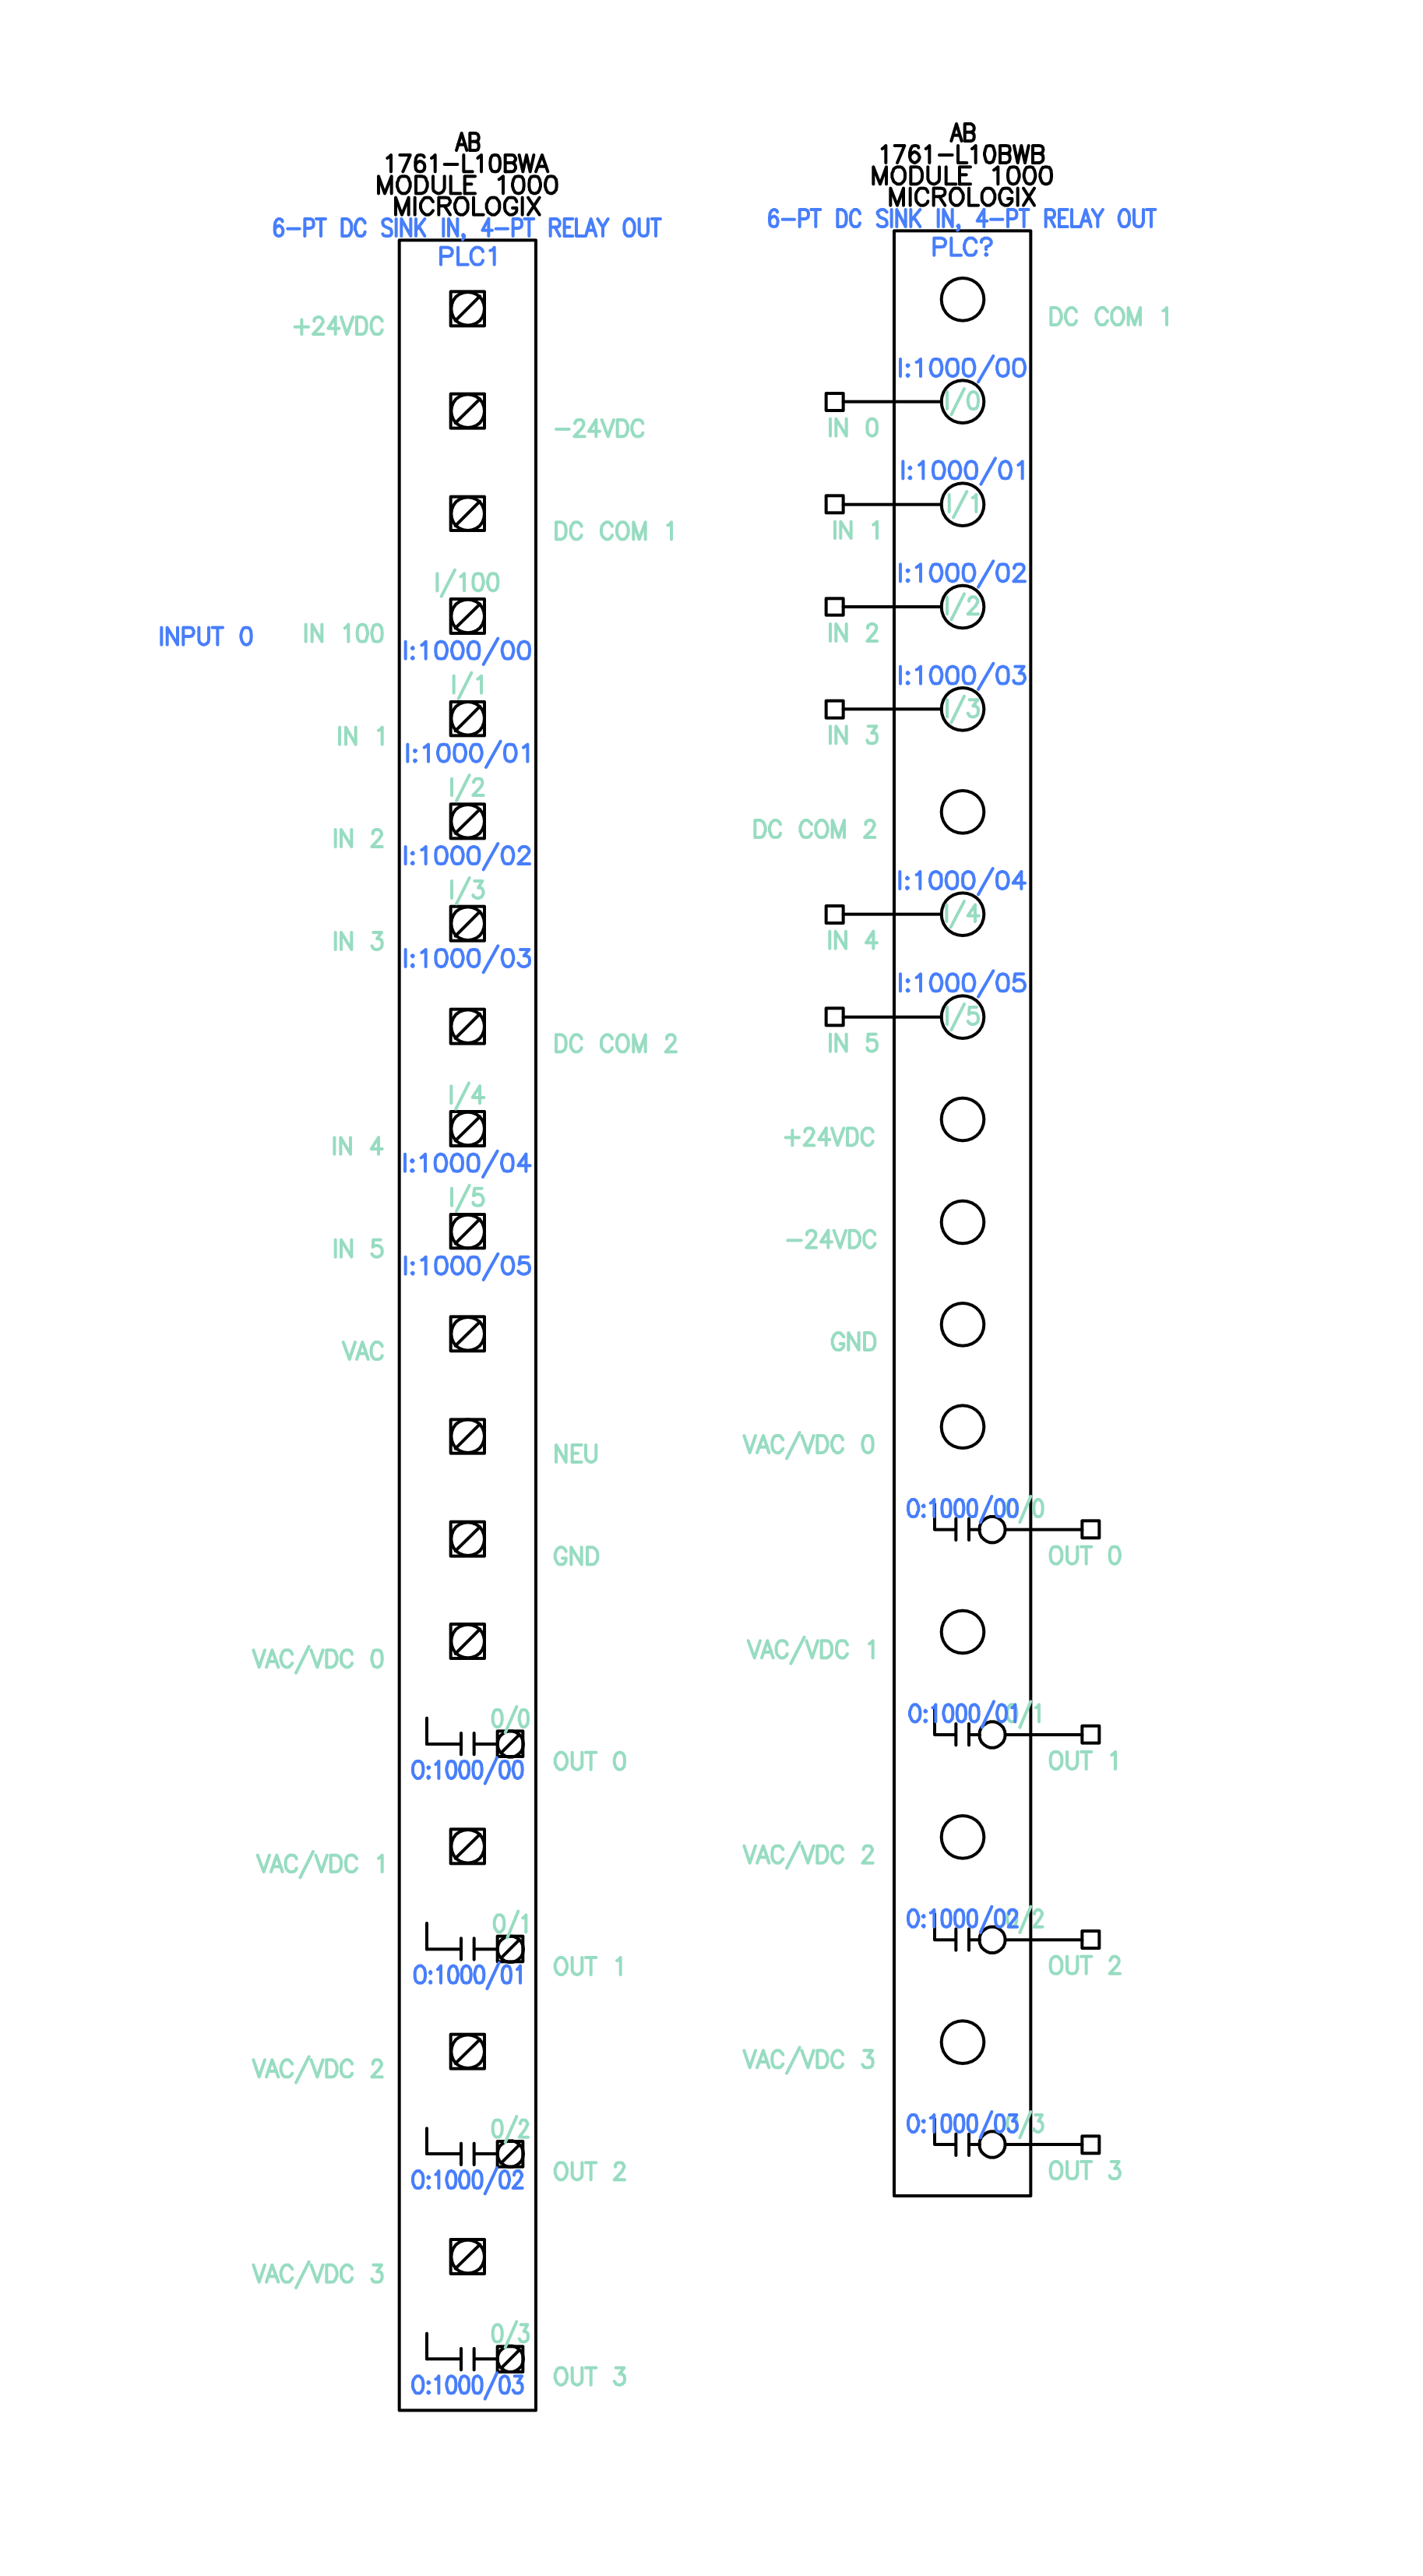
\includegraphics[width=.8\textwidth]{1.png}
    \caption{Inserting Parametric \& Full unit PLC}
    \label{fig:insert}
\end{figure}

\begin{figure}[H]
    \centering
    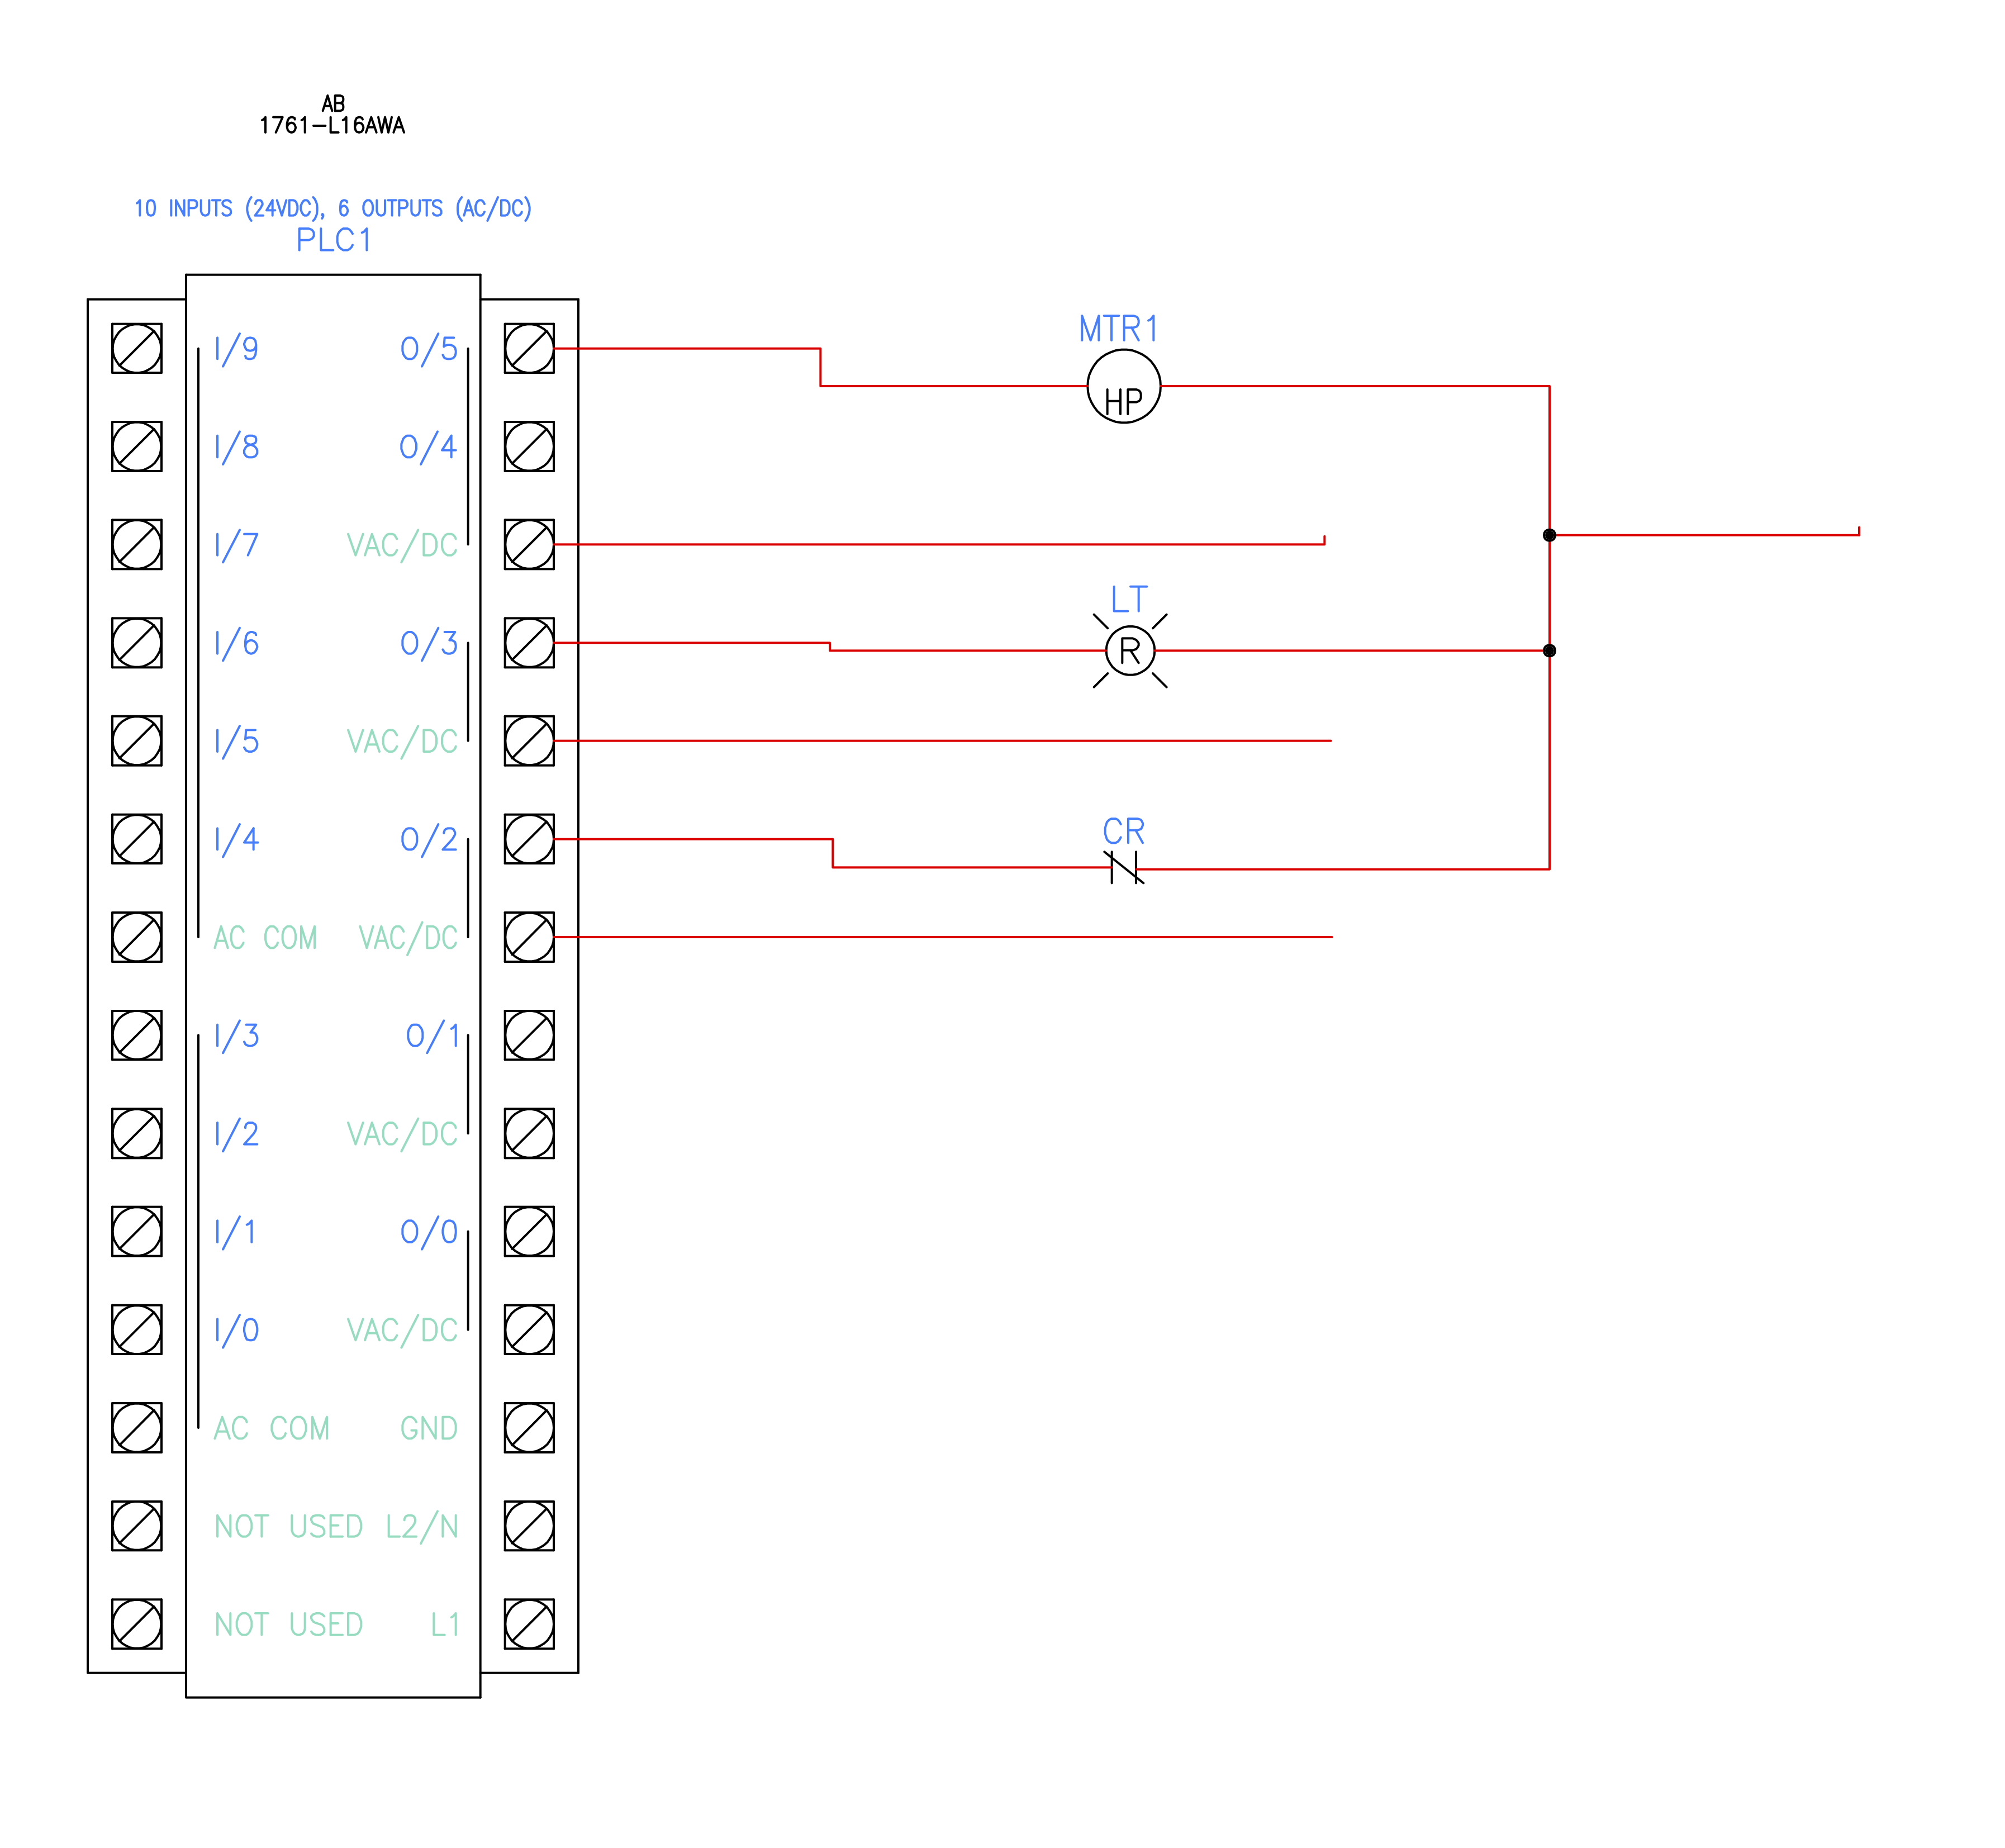
\includegraphics[width=\textwidth]{2.png}
    \caption{Editing \& modification of parametric \& full unit PLC}
    \label{fig:edit}
\end{figure}

\section*{Discussion \& Conclusion}
\addcontentsline{toc}{section}{Discussion \& Conclusion}
This experiment outlined the process of inserting, editing, and modifying a Parametric PLC. By configuring parameters and optimizing logic, we achieved efficient automation control. The ability to adjust PLC parameters enhances flexibility in real-world applications. In conclusion, understanding parametric PLC configuration is crucial for effective industrial automation. This lab reinforced practical skills in PLC programming and troubleshooting.
\\\\
The experiment is done following these video:\\
BD
Cinema mode
AutoCAD Electrical Bangla Tutorial Class - 14 How to Inserting Parametric \& Full Units PLC (https://www.youtube.com/watch?v=u1Mym8yr64Y)
\\
AutoCAD Electrical Bangla Tutorial Class - 15 How to Editing \& Modifying Parametric PLC (https://www.youtube.com/watch?v=nM-mSN8yfnA)

\bibliographystyle{IEEEtran}
\renewcommand{\bibname}{References}
\addcontentsline{toc}{section}{References}
\bibliography{ref}

\end{document}
